\documentclass[12pt,a4paper]{extarticle}

\usepackage[top=1.5in]{geometry}
\usepackage{amsmath}
\usepackage{graphicx}
\graphicspath{{images/}}

\title{\textbf{Computational Complexity Theory}}
\date{2 February 2017}
\author{Aniket Pandey}

\begin{document}
\maketitle

\section{Acknowledgement}
\textit{I would like to thank T. Aravind Reddy (B.Tech CSE) for mentoring me in the project and in helping me prepare this report. I would also like to thank ACA for giving me the opportunity to learn the topic in detail.}

\section{Introduction}
Computability and Complexity are the two facets of this topic. 
Although both are interconnected in some ways, my focus would be in the complexity part of the theory, to understand how efficient certain algorithms are in solving a problem. 
Major part of my study is primarily based on classifying the problems within certain Complexity Classes. 
For example, one of the very famous open questions in Theoretical Computer Science, \textbf{P} vs \textbf{NP} , which tries to differentiate between the complexity classes \textbf{P} (Polynomial Time) and \textbf{NP} (Non-deterministic Polynomial Time) is whether they are same or different.\\ \par Next, I'll discuss about Turing Machines , its working and how influencial it was in modern computing. There are different properties associated with Turing Machines, different terminologies and different types as well.Then finally I'll cover Cryptography and usefulness of Complexity Theory in cryptography. 

\section{Notations}
\subsection{Big-O Notation}
Big-O Notations are used in mathematics to characterize functions according to their growth rate. In Complexity Theory, efficiency of an algorithm is measured in terms of the input length $n$ as $n\rightarrow \infty $.\par Formal definition would be\\If $f:N\rightarrow N$ and $g:N\rightarrow N$ are two functions, then $f=$O$(g)$ if and only if $f(n)<c \cdot g(n)$ for a constant $c$ as $n\rightarrow\infty$.
\newpage
\subsection{Other Notations}
There are a few more notations which complement Big-O Notation. I will give a brief information about these.\par
For functions $f$ \& $g$ from $N$ to $N$

\begin{align}
f =&\:\Omega(g)\quad  \textrm{if} \,\,  g=O(f)\\
f =&\:\Theta(g)\quad \textrm{if} \,\,  f=O(g) \,\, \& \,\, g=O(f)\\
f =&\:o(g)\:\,\quad \textrm{if there exists }\varepsilon \textrm{ such that} \,\, f(n)<\varepsilon\cdot g(n) \\
f =&\:\omega(g)\quad \:\textrm{if} \,\,  g=o(f)
\end{align}

\section{Turing Machine}
\subsection{Computational Model}
Computational model is a set of operations which are used to measure the resources(time and space) that are needed for a certain problem ot be solved. In layman's terms, using this model , we can determine if the given algorithm is efficient or not. \par
One such model is \textit{Turing Machine} . It was invented by Alan Turing in $1936$. 
\subsection{Turing Machine}
\textit{Turing Machine} is an abstract machine which is made up of infinite tape(s) divided into discrete boxes called \textit{cells} and an imaginary head which can read the information in the boxes and can change the values of the cells. It also has a \textit{state register} which stores the information about the state of the head.\\
The basic \textit{Transition function} of a Turing Machine is defined as follows

\begin{equation}
\delta:Q\times\Gamma^k\longrightarrow Q\times\Gamma^{k-1}\times\{L,S,R\}^k
\end{equation}  

The above equation describes the functioning of a simple Turing Machine consisting of $k$ tapes where $1st$ tape is the input tape, the rest $k-1$ tapes are called \textit{work tapes}. Last one of them is designated as output tape.\par
Here, the input tape takes the input, the work tapes decide what to do with the input and in which direction to move the head. Then finally, changes(if any) are done in the output tape.\par
 
\subsubsection{Properties of Turing Machine} 
\begin{enumerate}
 \item If the time taken by a $k$ tape Turing Machine to compute a function is $T(n)$, where $T:N\rightarrow N$ is a Time-Constructible function. Then the time required to compute the same function by a single tape Turing Machine is $5kT(n)^2$.
 
 \newpage
 
 \item If a bi-directional Turing Machine computes a function in time $T(n)$, where $T:N\rightarrow N$ is a Time-Constructible function. Then the time required to compute the same function by a standard uni-directional Turing Machine is $4T(n)$.
\end{enumerate}

\subsubsection{Universal Turing Machine}
A Universal Turing Machine is a machine which can run an arbitrary Turing Machine for a given input. It is the most general form of Turing Machine, with the general form of Time complexity of UTM being $O(TlogT)$ where $T$ is for a normal TM . The reason I think it is because of the fact that a UTM has to deal with more bits of input than a normal one, which results in it being comparatively slower by a $log$ factor.\\\\
Another important result associated with a Universal Turing Machine is \textit{The Halting Problem}.The Halting Problem is a very interesting problem in context of \textit{Uncomputability}, which proves that we cannot have a UTM which can tell with certainty whether a Turing Machine will compute a program for a given input in a finite time. In simpler words, no machine can solve the Halting Problem. This is a very important result in Computer Science because most of the problems that we generally encounter are Halting Problems, that is, a solution to them would solve The Halting Problem.\par
Now since Halting Problem is unsolvable , it gives us another important result, that \textit{most problems are uncomputable}. For example, consider the \textit{Decision Problems} which can be considered to have input as an infinite set of either 0 or 1 ,i.e $\{0,1\}^*$ . Any combination of 0's and 1's is possible, so its impossible to compute it in finite time. Similarly, many such problems exist.\par

\section{Cryptography}
Crytpography, or encryption in modern terms is referred to the process of converting a normal message (plaintext) into an unintelligible text (ciphertext) using a key called encryption key. Reverse of the process, decryption uses decryption key to recover back the original message.

\begin{equation}
	D_k(E_k(x)) = x
\end{equation}

Here, 
\begin{align}
	E_k &=  \textrm{Encryption algorithm}  \\
	D_k &=  \textrm{Decryption algorithm}  \\
	x &=  \textrm{Plain text message}
\end{align}
\\\\
A Cipher is the pair of algorithms which govern the encryption and decryption of data. The secrecy of data relies on the fact that only the concerned party has the knowledge of cipher key. As shown in the image below, only Alice and Bob know the actual content. A particular eavesdropper, i.e Eve recovers the data being transmitted by Alice. But to her dismay, she will only have some gibberish in the data.  

\begin{center}
	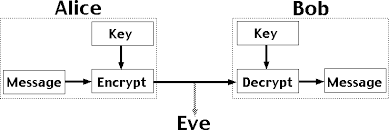
\includegraphics[width=12cm, height=6cm]{crypto}
\end{center}

\subsection{Public Key Cryptography}
The two keys, i.e Encryption and Decryption key, can either be public or private. But the frequently observed case is that the encryption cipher is public and decryption cipher is private.

This is also called \textbf{Asymmetric Cryptography}. \\

Public key Cryptography ensures confidentiality. That is, anyone will be able to encrypt their data but only the party with the private key will be able to decrypt it. 

\subsection{Perfect Secrecy}
  An Encryption algorithm, however complex, can be easily broken unless its perfectly secret. Perfect Secrecy relies on the condition that the ciphertext cannot be decrypted even if the decryption machine has unlimited computational power. \\
  
Perfect secrecy is like completely randomised ciphertext. There is no fixed rule that governs the encryption. The Encryption key is chosen by pseudorandom generators which are $ 100\% $ random. 

\subsubsection{One Time Pad}
 Just like Caeser shift, One time pad works on the principle of translating the letters by a certain length. However, the shift is not constant. For each letter in the original message, there is a unique encryption key. And that key is completely random, so the eavesdropper has no idea what the message is even after brute-forcing the cipher-text with unlimited computational power.
 
\subsubsection{Demonstration}
I will show a demonstration of how perfectly secret texts cannot be deciphered.\\

Suppose you want to encrypt a message BAD DOG with a One time pad XIF CLM (each letter chosen randomly). So after running the encryption algorithm..

\begin{center}
	(XIF CLM):(BAD DOG) $ \longrightarrow $  ZJJ GAT
\end{center}

Now, the eavesdropper will try to identify the pattern in the ciphertext. Since the encryption key was chosen completely randomly and is of the same length of the message, so there will not be any observable pattern in the text.  Using Brute force as the last resort, he'll try to get every possible feasible outcome. On trying out a few keys

\begin{center}
	(UIP DZZ):(ZJJ GAT) $ \longleftarrow $ EAT CAT\\
	(XIF CLM):(ZJJ GAT) $ \longleftarrow $  BAD DOG\\
	(TIP FMZ):(ZJJ GAT) $ \longleftarrow $ FAT ANT\\
\end{center}

Since, each of the decrypted messages EAT CAT, BAD DOG, FAT ANT have equal probability of being the original message, there is now way the eavesdropper will be certain of the actual message.

\end{document}
